\section{Numerical Examples}
\label{sec:ex}

In this section, we showcase GAIL's performance with two examples on
univariate function optimization and cubature.

\begin{example} We want to find the global minimum of the following functions: \scnote{Ping Sou-Cheng to help refine this example!}
\begin{align}
    f(x) &= -5 e^{-100(x-0.2)^2}-e^{ -100(x-1)^2}  \mbox{ for } x \in [0, 1.5], \label{eq1}
\\ f(x) &= \sin (10 \pi x^4 ) - x  \mbox{ for } x \in [0, 2]. \label{eq2}
\end{align}
In the case of (\ref{eq1}), \texttt{funmin\_g} automatically samples the
function more often in spiky areas and locates the global minimum
accurately. In contrast, MATLAB's \texttt{fminbnd} returns a local minimum.
In the case of (\ref{eq2}),we have a function that is increasingly
oscillating as $s$ increases and the true minimum occurs at the right
boundary point. \texttt{funmin\_g} is able to return an accurate
approximation, but \texttt{fminbnd} once again settles at a local minimum
far away from the global minimum.

We plot $f(x)$ and the global minima returned by \textbf{funmin\_g} and the
local minima by\texttt{funmin\_g}for the two given functions in
Figures~\ref{fig1} and \ref{fig2}. In addition, Table~\ref{tab1} summarizes the 
solver performance.

\begin{figure} % MATLAB Driver: min_pearc.m
\centering
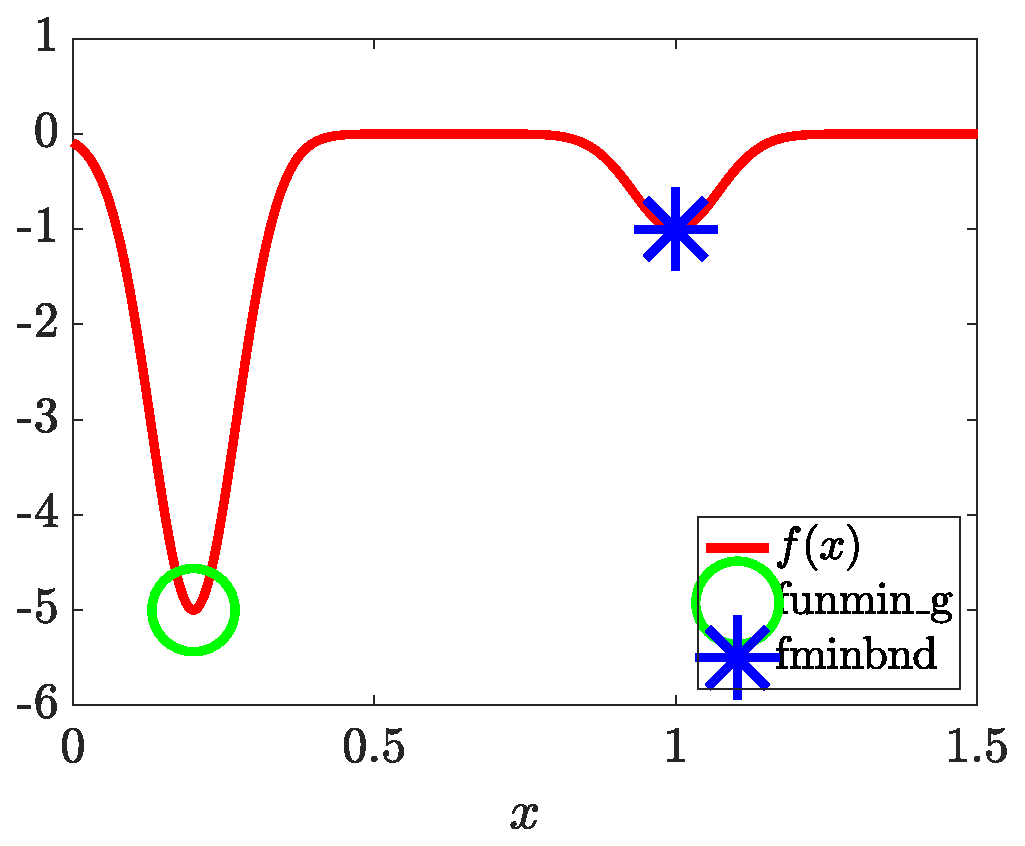
\includegraphics[width = 0.45\textwidth]{humps.eps} 
\caption{
This figure is reproducible by script \texttt{min\_pearc.m} in GAIL.}\label{fig1}
\end{figure}

\begin{figure} % MATLAB Driver: min_pearc.m
\centering
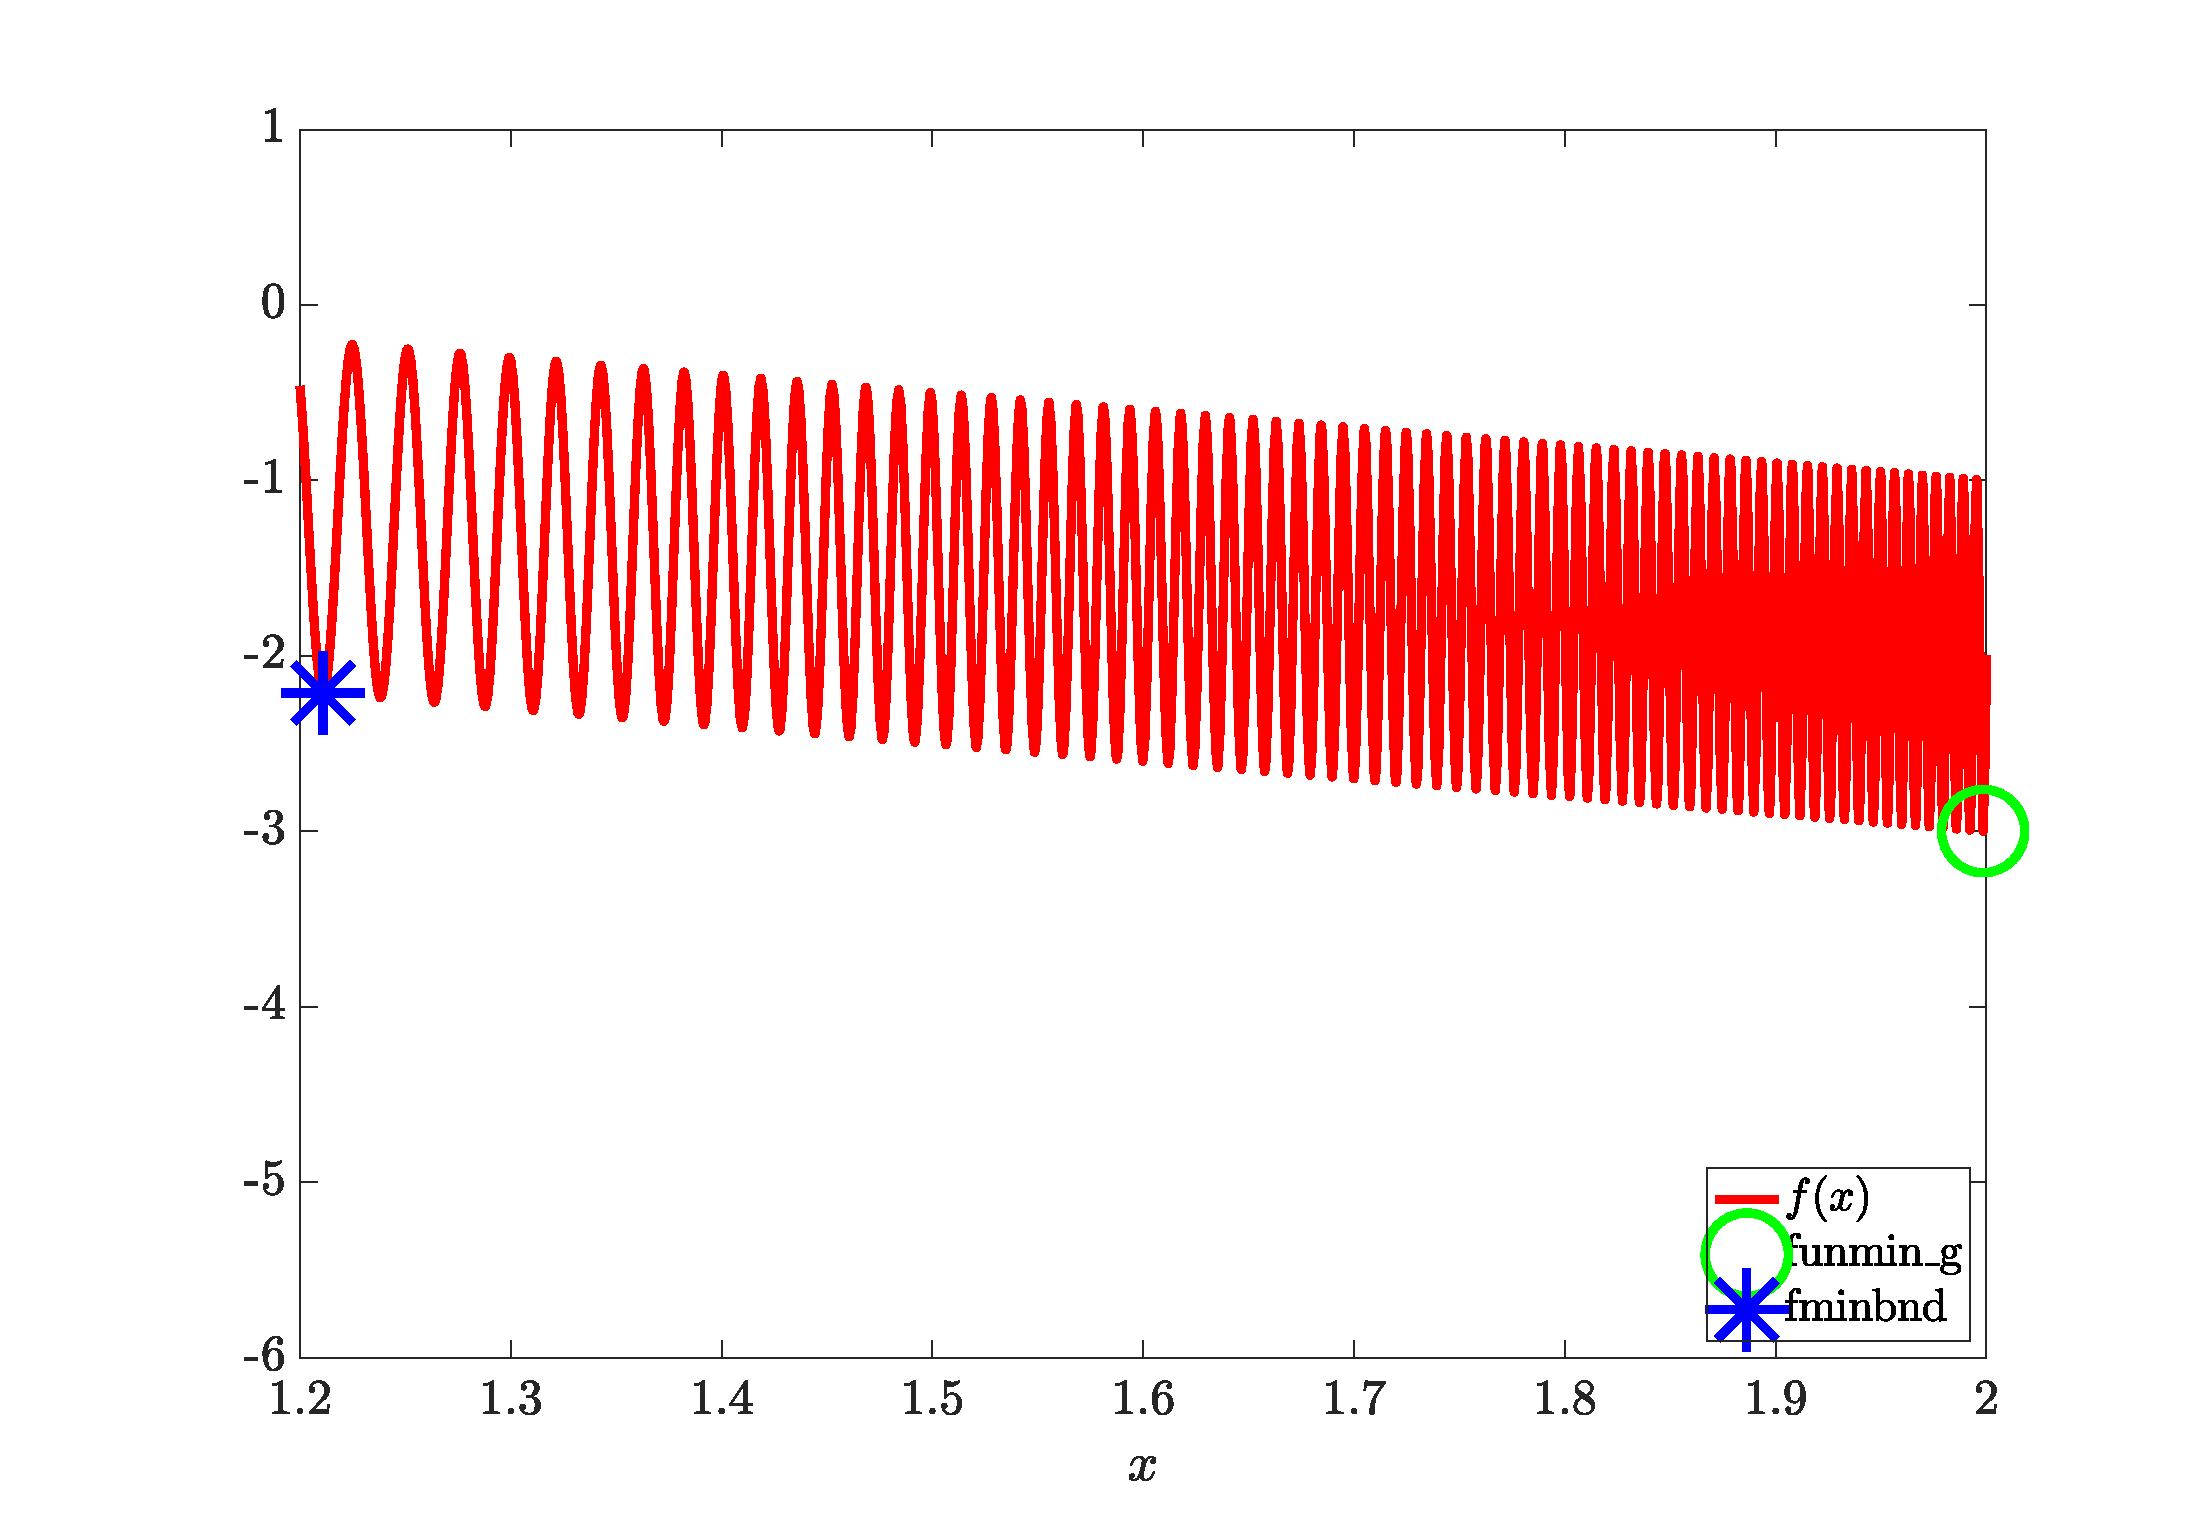
\includegraphics[width = 0.48\textwidth]{sine.eps} 
\caption{
This figure is reproducible by script \texttt{min\_pearc.m} in GAIL.}\label{fig2}
\end{figure}

\begin{table} % MATLAB Driver:  min_pearc.m
\centering
	\caption{Performance of \texttt{funmin\_g} and \texttt{fminbnd} with automatic stopping 
	criteria for optimizing functions defined in (\ref{eq1}) and (\ref{eq2}).
	These results can be  reproduced with  
	script \texttt{min\_pearc.m} in GAIL.
		\label{tab1}}
	$
    \begin{array}{l@{\qquad}r@{\quad}r@{\quad}r}
	\input{minPearcOut.txt} 
	\end{array}
	$
\end{table}
\end{example}


\begin{example}  In this example, we compare four (quasi-) Monte Carlo methods in GAIL in similar ways as
in Section~4 in \cite{hickernellmonte}.   \scnote{Sou-Cheng still working}

In Table~\ref{tab2}, we summarize the performance of the methods MC, Sobol,  Lattice, and Bayes---they
refer to the GAIL algorithms, \texttt{cubMC\_g}, \texttt{cubLattice\_g}, \texttt{cubSobol\_g},  \texttt{cubBayesLattice\_g}, respectively.
\begin{table} % MATLAB Driver: KeisterCubatureExamplePEARC.m
\centering
	\caption{Average performance of Monte Carlo algorithms with automatic stopping 
	criteria for estimating the integrals in \eqref{kei}
	for $1000$ independent runs. These results can be conditionally reproduced with  
	script \texttt{KeisterCubatureExamplePEARC.m} in GAIL.
	\label{tab2}}	 
	$
	%\arraycolsep=1.4pt\def\arraystretch{0.9}
    \begin{array}{l@{\qquad}r@{\quad}r@{\quad}r@{\quad}r@{\quad}r}
	\input{KeisterPearcOut.txt} 
	\end{array}
	$
\end{table}


\end{example} 









 
